% see https://en.wikibooks.org/wiki/LaTeX/Presentations

\documentclass{beamer}
\usepackage[utf8]{inputenc}
\usepackage{graphicx}

\definecolor{mfn_green}{HTML}{A1BF23}
\setbeamercolor{title}{fg=black}
\setbeamerfont{title}{family=\sffamily,series=\bf,size=\Large}
\setbeamercolor{frametitle}{fg=mfn_green}
\setbeamerfont{subtitle}{family=\sffamily,shape=\itshape}
%Running wikis at the Museum with Docker: past, present and future The Museum outputs exhibitions, science papers, conferences, and so much more. None of this would be %possible without cooperation between researchers, designers, organizers and of course admins and developers. Wikis were introduced at the Museum in 2014 as an %experiment to improve  cooperation within project teams. I'll talk about how Docker solves many of the problems of running a bunch of wikis on a string, and also %about pending questions we are currently trying to answer.
%I am a computer scientist and joined the Museum in 2014. I have worked at the Technische Universität Berlin and at Waag Technology & Society in Amsterdam.


\title
{Running wikis at the Museum with Docker}
\subtitle{past, present and future}
\author
{Alvaro Ortiz-Troncoso\inst{1}}
\institute % (optional)
{
  \inst{1}%
  Museum für Naturkunde Berlin
}
\date
{Docker Meetup at Museum für Naturkunde Berlin, 2018}
\subject{Computer Science}

\begin{document}
{
  \usebackgroundtemplate {
    \vbox to 30mm{\vfil\hbox to \paperwidth{\hfil
\includegraphics[width=30mm]{mfn_logo_klein.png}}\vfil}
  }
  \frame{\titlepage}
}

% The Museum
\begin{frame}
  \frametitle{Das Museum / The Museum}
  \begin{figure}
  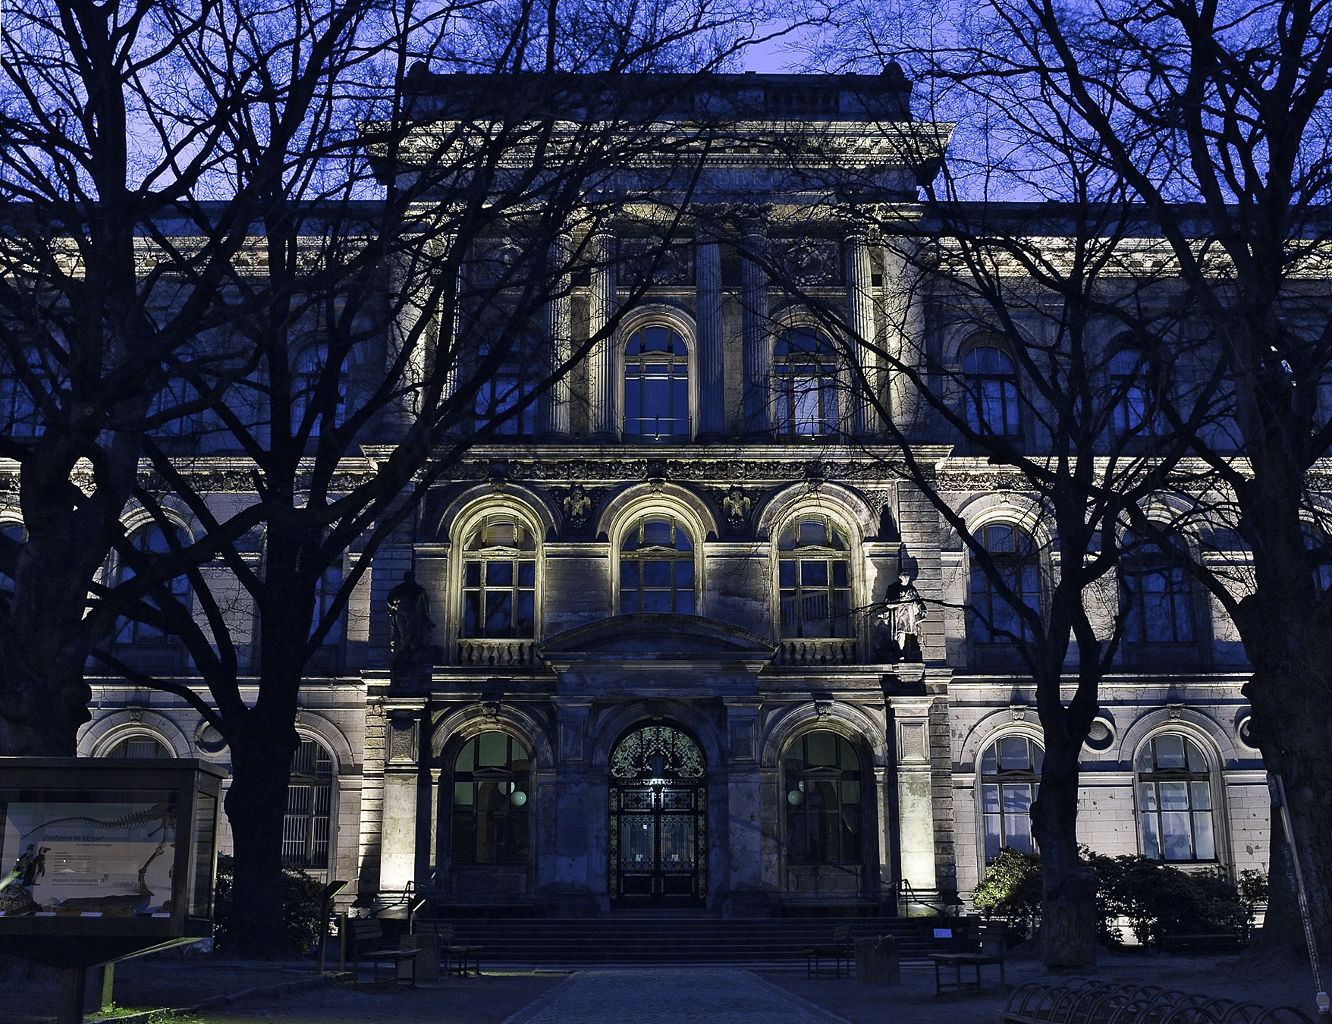
\includegraphics[width=100mm]{Gebaeude_Nacht.jpg}
  \end{figure}
\end{frame}

\begin{frame}
  \frametitle{Das Museum / The Museum}
  \begin{figure}
  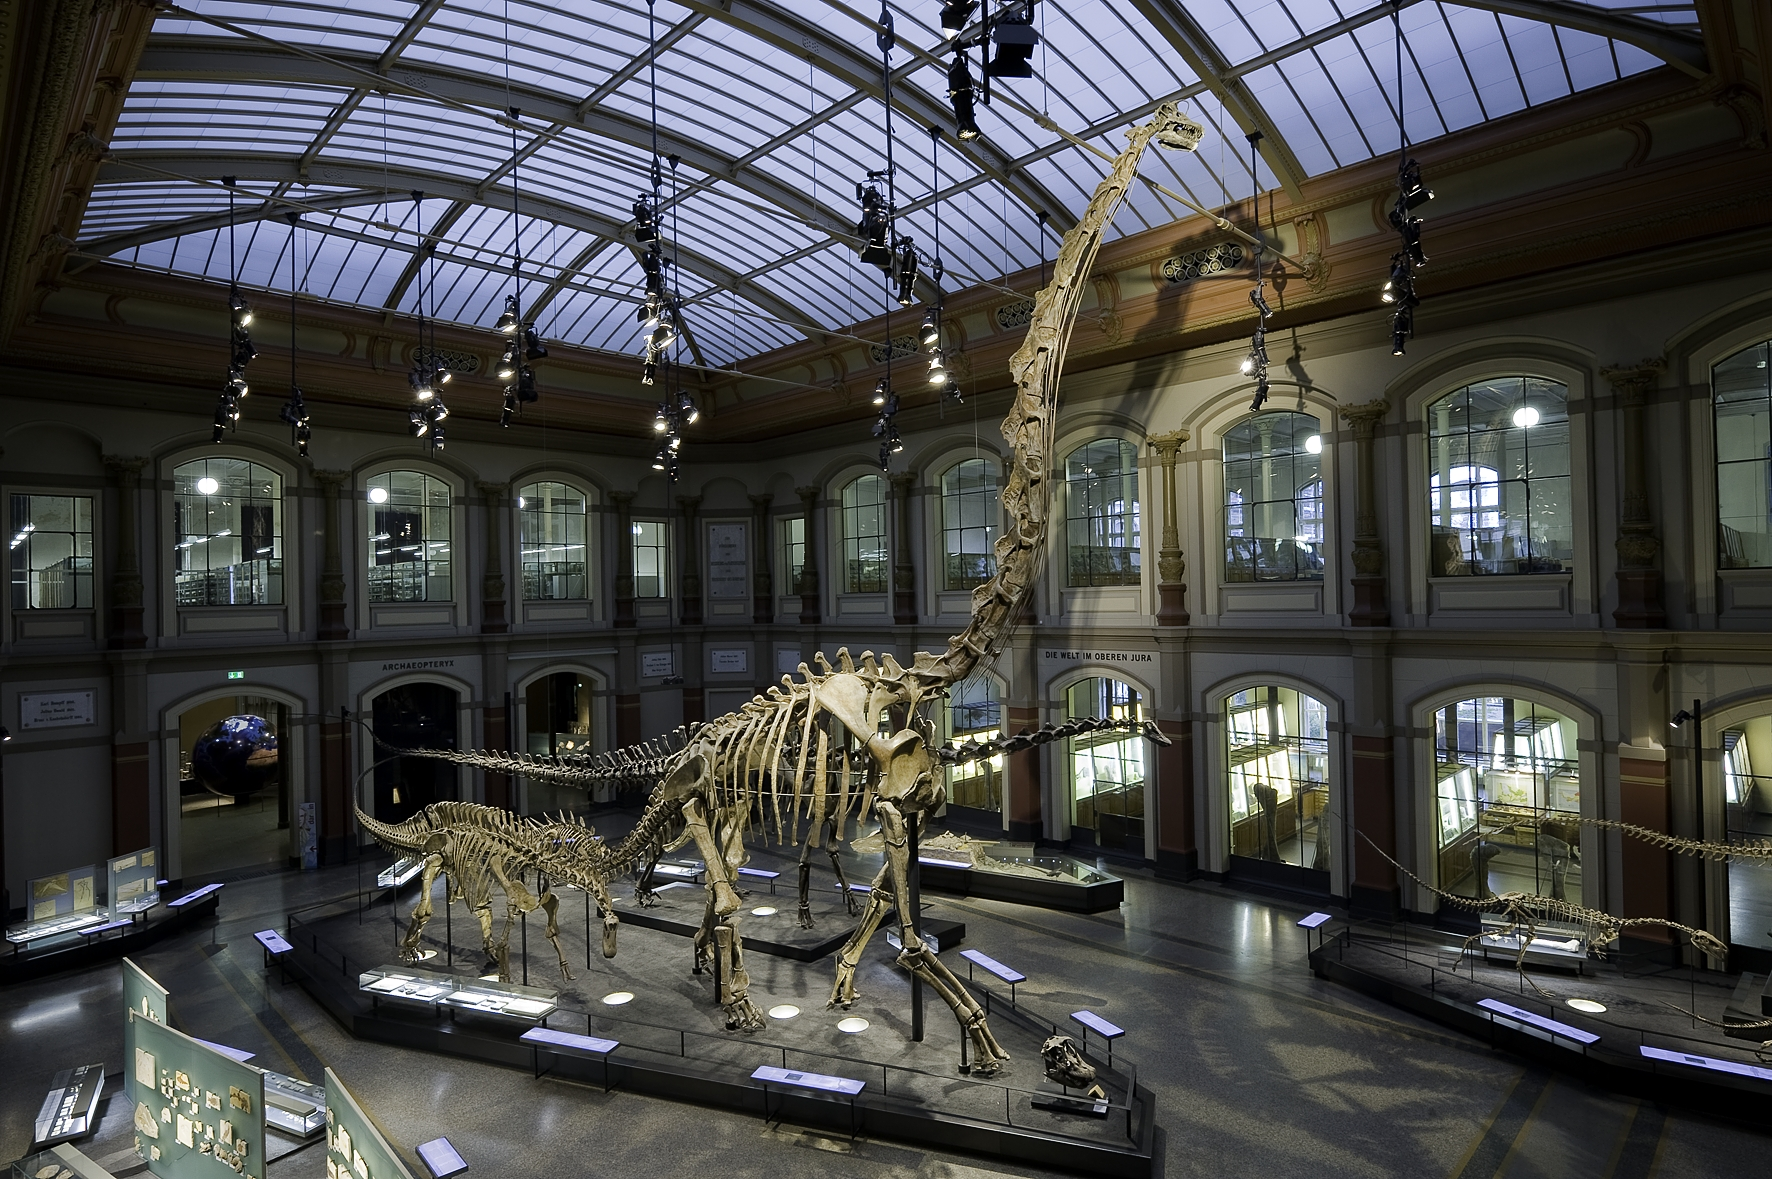
\includegraphics[width=100mm]{Brachiosaurus_02_15cm.jpg}
  \end{figure}
\end{frame}

\begin{frame}
  \frametitle{Das Museum / The Museum}
  \begin{figure}
  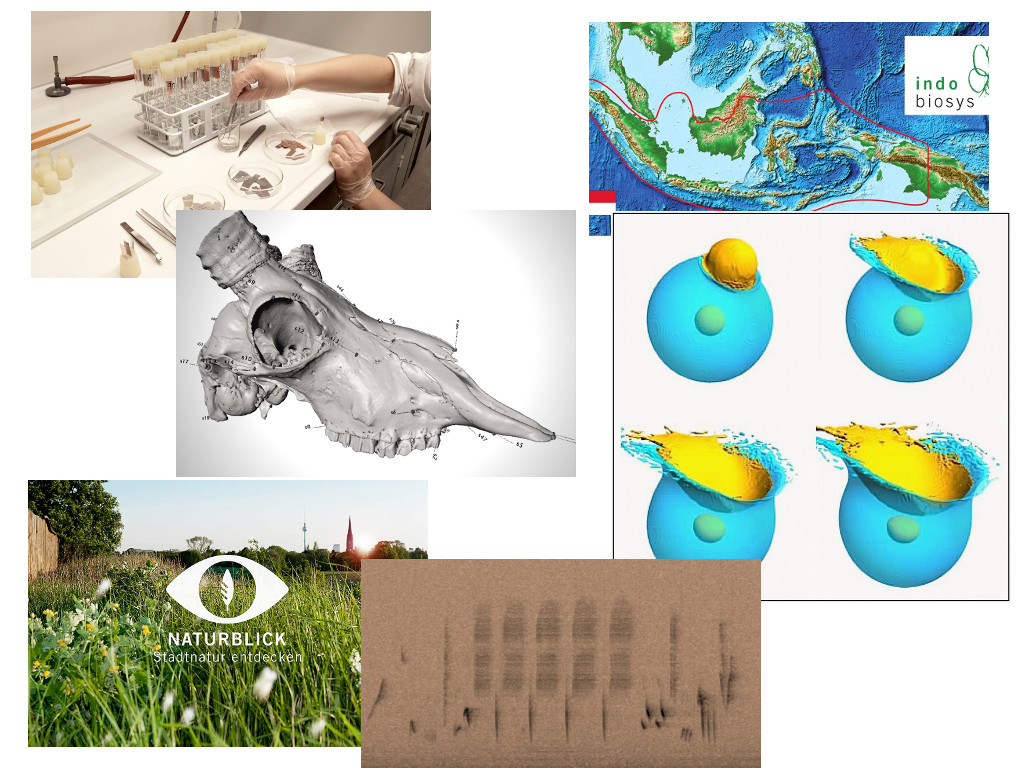
\includegraphics[width=100mm]{Forschung.jpg}
  \end{figure}
\end{frame}

% The past
\begin{frame}
  \frametitle{This is the first slide}
  % Content goes here
\end{frame}

% The present
\begin{frame}
  \frametitle{This is the first slide}
  % Content goes here
\end{frame}

% The future
\begin{frame}
  \frametitle{This is the first slide}
  % Content goes here
\end{frame}


\end{document}


